\documentclass[a4paper,11pt]{jarticle}

% レイアウト
\setlength{\hoffset}{0cm}
\setlength{\oddsidemargin}{-3mm}
\setlength{\evensidemargin}{-3cm}
\setlength{\marginparsep}{0cm}
\setlength{\marginparwidth}{0cm}
\setlength{\textheight}{24.7cm}
\setlength{\textwidth}{17cm}
\setlength{\topmargin}{-45pt}


\renewcommand{\baselinestretch}{1.2}
\renewcommand{\floatpagefraction}{1}
\renewcommand{\topfraction}{1}
\renewcommand{\bottomfraction}{1}
\renewcommand{\textfraction}{0}
\renewcommand\thefootnote{\arabic{footnote})}

% パッケージ
\usepackage[dvipdfmx]{graphicx}
\usepackage{amsmath,amssymb,epsfig}
\usepackage{eucal}
\usepackage{bm}
\usepackage{ascmac}
\usepackage{pifont}
\usepackage{multirow}
\usepackage{enumerate}
\usepackage{cases}
\usepackage{type1cm}
\usepackage{cancel}
\usepackage{url}
\usepackage{cite}
%\usepackage{color}
\usepackage[dvipdfmx]{color}
\usepackage{caption}
\usepackage[caption=false]{subfig}
\captionsetup[figure]{labelsep=space}
\usepackage{here}

% 擬似コード作成用
\usepackage[ruled,vlined]{algorithm2e}
\usepackage{setspace}
\DeclareRelationFont{JY1}{mc}{it}{}{OT1}{cmr}{it}{}
\DeclareRelationFont{JT1}{mc}{it}{}{OT1}{cmr}{it}{}
\DeclareFontShape{JY1}{mc}{m}{it}{<5> <6> <7> <8> <9> <10> sgen*min
    <10.95><12><14.4><17.28><20.74><24.88> min10
    <-> min10}{}
\DeclareFontShape{JT1}{mc}{m}{it}{<5> <6> <7> <8> <9> <10> sgen*tmin
    <10.95><12><14.4><17.28><20.74><24.88> tmin10
    <-> tmin10}{}
\DeclareRelationFont{JY1}{mc}{sl}{}{OT1}{cmr}{sl}{}
\DeclareRelationFont{JT1}{mc}{sl}{}{OT1}{cmr}{sl}{}
\DeclareFontShape{JY1}{mc}{m}{sl}{<5> <6> <7> <8> <9> <10> sgen*min
    <10.95><12><14.4><17.28><20.74><24.88> min10
    <-> min10}{}
\DeclareFontShape{JT1}{mc}{m}{sl}{<5> <6> <7> <8> <9> <10> sgen*tmin
    <10.95><12><14.4><17.28><20.74><24.88> tmin10
    <-> tmin10}{}
\DeclareRelationFont{JY1}{mc}{sc}{}{OT1}{cmr}{sc}{}
\DeclareRelationFont{JT1}{mc}{sc}{}{OT1}{cmr}{sc}{}
\DeclareFontShape{JY1}{mc}{m}{sc}{<5> <6> <7> <8> <9> <10> sgen*min
    <10.95><12><14.4><17.28><20.74><24.88> min10
    <-> min10}{}
\DeclareFontShape{JT1}{mc}{m}{sc}{<5> <6> <7> <8> <9> <10> sgen*tmin
    <10.95><12><14.4><17.28><20.74><24.88> tmin10
    <-> tmin10}{}
\DeclareRelationFont{JY1}{gt}{it}{}{OT1}{cmbx}{it}{}
\DeclareRelationFont{JT1}{gt}{it}{}{OT1}{cmbx}{it}{}
\DeclareFontShape{JY1}{mc}{bx}{it}{<5> <6> <7> <8> <9> <10> sgen*goth
    <10.95><12><14.4><17.28><20.74><24.88> goth10
    <-> goth10}{}
\DeclareFontShape{JT1}{mc}{bx}{it}{<5> <6> <7> <8> <9> <10> sgen*tgoth
    <10.95><12><14.4><17.28><20.74><24.88> tgoth10
    <-> tgoth10}{}
\DeclareRelationFont{JY1}{gt}{sl}{}{OT1}{cmbx}{sl}{}
\DeclareRelationFont{JT1}{gt}{sl}{}{OT1}{cmbx}{sl}{}
\DeclareFontShape{JY1}{mc}{bx}{sl}{<5> <6> <7> <8> <9> <10> sgen*goth
    <10.95><12><14.4><17.28><20.74><24.88> goth10
    <-> goth10}{}
\DeclareFontShape{JT1}{mc}{bx}{sl}{<5> <6> <7> <8> <9> <10> sgen*tgoth
    <10.95><12><14.4><17.28><20.74><24.88> tgoth10
    <-> tgoth10}{}
\DeclareRelationFont{JY1}{gt}{sc}{}{OT1}{cmbx}{sc}{}
\DeclareRelationFont{JT1}{gt}{sc}{}{OT1}{cmbx}{sc}{}
\DeclareFontShape{JY1}{mc}{bx}{sc}{<5> <6> <7> <8> <9> <10> sgen*goth
    <10.95><12><14.4><17.28><20.74><24.88> goth10
    <-> goth10}{}
\DeclareFontShape{JT1}{mc}{bx}{sc}{<5> <6> <7> <8> <9> <10> sgen*tgoth
    <10.95><12><14.4><17.28><20.74><24.88> tgoth10
    <-> tgoth10}{}
\DeclareRelationFont{JY1}{gt}{it}{}{OT1}{cmr}{it}{}
\DeclareRelationFont{JT1}{gt}{it}{}{OT1}{cmr}{it}{}
\DeclareFontShape{JY1}{gt}{m}{it}{<5> <6> <7> <8> <9> <10> sgen*goth
    <10.95><12><14.4><17.28><20.74><24.88> goth10
    <-> goth10}{}
\DeclareFontShape{JT1}{gt}{m}{it}{<5> <6> <7> <8> <9> <10> sgen*tgoth
    <10.95><12><14.4><17.28><20.74><24.88> tgoth10
    <-> tgoth10}{}
\endinput
%%%% end of jdummy.def

% カウンタの設定
\setcounter{section}{0}
\setcounter{subsection}{0}
\setcounter{subsubsection}{0}
\setcounter{equation}{0}

% キャプションの図をFigに変更
\renewcommand{\figurename}{Fig.}
\renewcommand{\tablename}{Tab.}

% 式番号を式(章番号.番号)に
\makeatletter
\renewcommand{\theequation}{\arabic{equation}}
\@addtoreset{equation}{section}
\makeatother

% タイトル部分
\title{\vspace{-20truemm}
{\normalsize \rightline{平成29年\ 10月\ 18日}}
{\large 確率システム制御特論\\}
第2回演習問題\\
\date{}
\vspace{-2truemm}}
\author{機械知能工学専攻 知能制御工学コース \hspace{3mm} 17344219 \ 二宮 悠二}
%---------------------------------------------
% ドキュメントの開始
\begin{document}
\parindent = 0pt % 字下げoff
% 表紙
\titlepage
\maketitle
%---------------------------------------------
% 課題内容
{\Large{\bf 問題}}
%---------------------------------------------
\begin{enumerate}
 \item 次の状態方程式で記述される時系列$ \{ y(k) \} $をARMAモデルに変換せよ.
%-----------------------------------
       \begin{equation}
	\left[
	 \begin{array}{c}
	  x_1(k+1) \\
	  x_2(k+1) \\
	 \end{array}
	\right] = \left[
		  \begin{array}{cc}
		   -0.7 & 0 \\
		   0 & -0.3 \\
		  \end{array}
		  \right]
	\left[
	\begin{array}{c}
	 x_1(k) \\
	 x_2(k) \\
	\end{array}
	\right] + \left[
		  \begin{array}{c}
		   1 \\
		   1 \\
		  \end{array}
		  \right] v(k)
	\label{status}
       \end{equation}
%-----------------------------------
       \begin{equation}
		y(k) = \left[
	       \begin{array}{cc}
		-2 & 3 \\
	       \end{array}
	       \right] \left[
		       \begin{array}{c}
			x_1(k) \\
			x_2(k)\\
		       \end{array}
		       \right]
	\label{output}
       \end{equation}
%-----------------------------------

 \item 一括処理最小二乗法の適用により,1次元の時系列データを自らで7点以上定め,二次のARモデルのパラメータを推定せよ.\\
%-----------------------------------
       \begin{equation}
	y(k) = - a_1y(k-1) - a_2y(k-2) + v(k),~~ k = 1,2,\cdots, N
       \end{equation}
\label{3}
\end{enumerate}
%-----------------------------------
%---------------------------------------------
{\Large{\bf 解答}}
%---------------------------------------------
\begin{enumerate}
 \item 
\ \ (\ref{status}),(\ref{output})式を,それぞれ初期値を$ 0 $として$ z $変換すると次のようになる.
%-----------------------------------
\begin{equation}
 \left[
  \begin{array}{c}
   z x_1(z) \\
   z x_2(z) \\
  \end{array}
 \right] = \left[
 \begin{array}{cc}
  -0.7 & 0 \\
  0 & -0.3 \\
 \end{array}
	   \right]
 \left[
  \begin{array}{c}
   x_1(z) \\
   x_2(z) \\
  \end{array}
 \right] + \left[
 \begin{array}{c}
  1 \\
  1 \\
 \end{array}
	   \right] v(k)
 \label{4}
\end{equation}
%-----------------------------------
\begin{equation}
 y(z) = \left[
	 \begin{array}{cc}
	  -2 & 3 \\
	 \end{array}
	\right] \left[
	\begin{array}{c}
	 x_1(z) \\
	 x_2(z)\\
	\end{array}
		\right]
\label{5}
\end{equation}
%-----------------------------------
ただし,$ x_1(z), ~ x_2(z), ~ v(z), ~ y(z) $はそれぞれ$ x_1(k), ~ x_2(k), ~ v(k), ~ y(k) $の$ z $変換である.(\ref{4})式をまとめると次のようになる.
%-----------------------------------
\begin{equation}
 \left[
  \begin{array}{c}
   x_1(z) \\
   x_2(z) \\
  \end{array}
 \right] = \left[
 \begin{array}{cc}
  z + 0.7 & 0 \\
  0 & z + 0.3 \\
 \end{array}
	   \right]^{-1} \left[
	   \begin{array}{c}
	    1 \\
	    1
	   \end{array}
			\right] v(z)
 \label{6}
\end{equation}
%-----------------------------------
(\ref{5}),(\ref{6})式より次式を得る.
%-----------------------------------
\begin{eqnarray}
 y(z) & = & \left[
	 \begin{array}{cc}
	  -2 & 3
	 \end{array}
	\right] \left[ \begin{array}{cc}
	 z + 0.7 & 0 \\
	 0 & z + 0.3
	\end{array}
		\right]^{-1} \left[
			     \begin{array}{c}
			      1 \\
			      1
			     \end{array}
			     \right] v(z) \nonumber \\
 & = & \dfrac{z + 1.5}{( z + 0.7 )( z + 0.3 )}v(z) \nonumber \\
 & = & \dfrac{z + 1.5}{z^2 + z + 0.21} v(z) \nonumber \\
 & = & \dfrac{z^{-1} + 1.5z^{-2}}{1 + z^{-1} + 0.21^{-2}} v(z)
\end{eqnarray}
%-----------------------------------
\ \ 以上より,与式をARMAモデルへ変換することができた.
%---------------------------------------------
 \item
\ \ まず,与式(\ref{3})を次のように変形する.
%-----------------------------------
\begin{equation}
 y(k) = \mbox{\boldmath$\theta$}^T \mbox{\boldmath$\varphi$}(k) + v(k)
\end{equation}
%-----------------------------------
ただし,
%-----------------------------------
\begin{eqnarray}
 \mbox{\boldmath$\theta$} & = & \left[ ~ a_1 ~~ a_2 ~ \right]^T \\
 \mbox{\boldmath$\varphi$}(k) & = & \left[ ~ -y(k-1) ~~ -y(k-2) ~ \right]^T
\end{eqnarray}
%-----------------------------------
であり,$ \mbox{\boldmath$\theta$} $は未知パラメータベクトル,$ \mbox{\boldmath$\varphi$}(k) $は回帰ベクトルと呼ばれる.ARモデルでは未知パラメータに関して線形な形で時系列$ y(k) $を記述でき,パラメータ推定のための評価関数として次式を採用する.
%-----------------------------------
\begin{eqnarray}
 J_N & = &  \dfrac{1}{N} \sum^N_{k=1} \left\{ y(k) - \widehat{\mbox{\boldmath$\theta$}}^T \mbox{\boldmath$\varphi$}(k) \right\}^2 \nonumber \\
     & = & \dfrac{1}{N} \sum^N_{k=1} \left( y^2(k) - 2\widehat{\mbox{\boldmath$\theta$}}^T \mbox{\boldmath$\varphi$}(k) y(k) + \widehat{\mbox{\boldmath$\theta$}}^T \mbox{\boldmath$\varphi$}(k) \mbox{\boldmath$\varphi$}^T(k) \widehat{\mbox{\boldmath$\theta$}} \right) \nonumber \\
     & = & \dfrac{1}{N} \sum^N_{k=1} y^2(k) - 2 \widehat{\mbox{\boldmath$\theta$}}^T \left(\dfrac{1}{N} \sum^N_{k=1} \mbox{\boldmath$\varphi$}(k) y(k) \right) + \widehat{\mbox{\boldmath$\theta$}}^T \left(\dfrac{1}{N} \sum^N_{k=1} \mbox{\boldmath$\varphi$}(k) \mbox{\boldmath$\varphi$}^T(k) \right) \widehat{\mbox{\boldmath$\theta$}}
\end{eqnarray}
%-----------------------------------
この式を最小とするための$ ~ \widehat{\mbox{\boldmath$\theta$}} = \left[ ~ \widehat{a}_1 ~~ \widehat{a}_2 ~ \right]^T $をパラメータ推定値とする.ここで,
%-----------------------------------
\begin{equation}
 c_N = \dfrac{1}{N} \sum^N_{k=1}y^2(k), ~~ \mbox{\boldmath$h$}_N = \dfrac{1}{N} \sum^N_{k=1} \mbox{\boldmath$\varphi$}(k) y(k), ~~ \mbox{\boldmath$G$}_N = \dfrac{1}{N} \sum^N_{k=1} \mbox{\boldmath$\varphi$}(k) \mbox{\boldmath$\varphi$}^T(k)
\label{12}
\end{equation}
%-----------------------------------
とおくと,(11)式は次のようになる.
%-----------------------------------
\begin{equation}
 J_N = \widehat{\mbox{\boldmath$\theta$}}^T \mbox{\boldmath$G$}_N \widehat{\mbox{\boldmath$\theta$}} - 2\widehat{\mbox{\boldmath$\theta$}}^T \mbox{\boldmath$h$}_N + c_N
\end{equation}
%-----------------------------------
これは,パラメータベクトル$ \widehat{\mbox{\boldmath$\theta$}} $に関して二次形式であり,行列$ \mbox{\boldmath$G$}_N $が正定値であればこの評価関数$ J_N $は最小値を持つ.そこで,$ J_N $を$ \widehat{\mbox{\boldmath$\theta$}} $に関して微分して$ 0 $とおき,これについて解くと,
%-----------------------------------
\begin{equation}
 \dfrac{{\rm d}J_N}{{\rm d}\widehat{\mbox{\boldmath$\theta$}}} = 2\mbox{\boldmath$G$}_N \widehat{\mbox{\boldmath$\theta$}} - 2\mbox{\boldmath$h$}_N = 0
\end{equation}
%-----------------------------------
より,一括処理最小二乗推定法の式
%-----------------------------------
\begin{eqnarray}
 \mbox{\boldmath$G$}_N \widehat{\mbox{\boldmath$\theta$}} & = & \mbox{\boldmath$h$}_N \nonumber \\
 \widehat{\mbox{\boldmath$\theta$}} & = & \mbox{\boldmath$G$}_N^{-1} \mbox{\boldmath$h$}_N
\end{eqnarray}
%-----------------------------------
を得る.\\
\ \ 時系列データとして,{\bf Tab.}{\ref{values}}を利用した\cite{data}.この中から連続する7点を使用する.具体的には,$ y(k-2) $の値が必要となるため,$ k = 1 $を$ {\rm No.} 3 $に設定する.数値を(12)式へ代入して解くと次のようになる.
%-----------------------------------
\begin{table}[b]
  \begin{center}
    \caption{推定パラメータの導出に用いたセンサの値}
    \begin{tabular}{c|c} \hline
      No. & センサ値 \\ \hline \hline
      1 & 3030.93 \\ \hline
      2 & 3095.78 \\ \hline
      3 & 2932.61 \\ \hline
      4 & 2988.72 \\ \hline
      5 & 3032.24 \\ \hline
      6 & 2946.25 \\ \hline
      7 & 3030.27 \\ \hline
      8 & 3058.88 \\ \hline
      9 & 2967.68 \\ \hline
      10 & 3016.11 \\ \hline
    \end{tabular}
    \label{values}
  \end{center}
\end{table}
%-----------------------------------
%-----------------------------------
\begin{eqnarray}
 \mbox{\boldmath$G$}_7 & = & \dfrac{1}{7} \sum^7_{k=1} \left[
						       \begin{array}{cc}
							y^2(k-1) & y(k-1) y(k-2) \\
							y(k-1) y(k-2) & y^2(k-2)
						       \end{array}\right] \nonumber \\
                       & = & \left[
			     \begin{array}{cc}
			      9075810 & 9060000 \\
			      9060000 & 9051490
			     \end{array}\right] \\
 \mbox{\boldmath$h$}_7 & = & \dfrac{1}{7} \sum^7_{k=1} \left[
						   \begin{array}{c}
						    -y(k)y(k-1) \\
						    -y(k)y(k-2)
						   \end{array}\right] \nonumber \\
                       & = & \left[
			     \begin{array}{c}
			      -9016380 \\
			      -9004640
			     \end{array}
			     \right]
\end{eqnarray}
%-----------------------------------
したがって,ARモデルの推定パラメータは
%-----------------------------------
\begin{eqnarray}
 \widehat{\mbox{\boldmath$\theta$}} & = & \left[
					   \begin{array}{cc}
					    \widehat{a}_1 & \widehat{a}_2 \\
					   \end{array}
					     \right]^T \nonumber \\
                                    & = & \mbox{\boldmath$G$}_7^{-1} \mbox{\boldmath$h$}_7 \nonumber \\
                                    & = & \left[
					   \begin{array}{cc}
					    9075810 & 9060000 \\
					    9060000 & 9051490
					   \end{array}
					  \right]^{-1} \left[
					  \begin{array}{c}
					   -9016380 \\
					   -9004640
					  \end{array}
						       \right] \nonumber \\
                                    & = & \left[
					  \begin{array}{c}
					   -4.008 \times 10^{-5} \\
					   -4.868 \times 10^{-5}
					  \end{array}
					  \right]
\end{eqnarray}
%-----------------------------------
となる.

\end{enumerate}
% % 図の挿入

% \begin{figure}[b]
%  \begin{center}
%   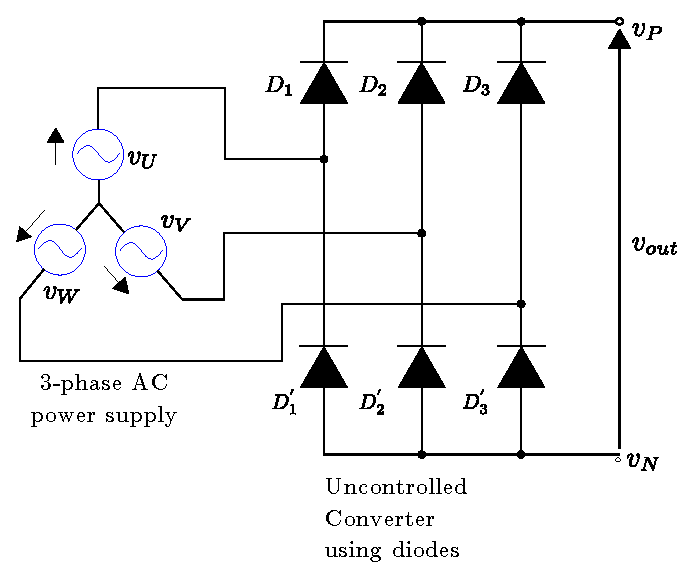
\includegraphics[scale=0.9]{../figure/circuit.eps}
%   \caption{Uncontrolled converter}
%   \label{circuit}
%  \end{center}
% \end{figure}


% % 表の挿入

% \begin{table}[htb]
%   \begin{center}
%     \caption{各素子のパラメータ}
%     \begin{tabular}{c|c|c} \hline
%       定数名[単位] & 記号 & 値 \\ \hline \hline
%       周波数[Hz] & $f_U,f_V,f_W$ & 120 \\ \hline
%                      & $\phi_U$ & $\frac{2\pi}{3}$ \\
%       初期位相角[rad] & $\phi_V$ & $\frac{4\pi}{3}$ \\
%                      & $\phi_W$ & $2\pi$ \\ \hline
%       抵抗[$\Omega$] & $R$ & 10 \\ \hline
%     \end{tabular}
%     \label{param}
%   \end{center}
% \end{table}


% % 図の挿入

% \begin{figure}[tb]
%  \centering
%  \vspace{0.5cm}
%  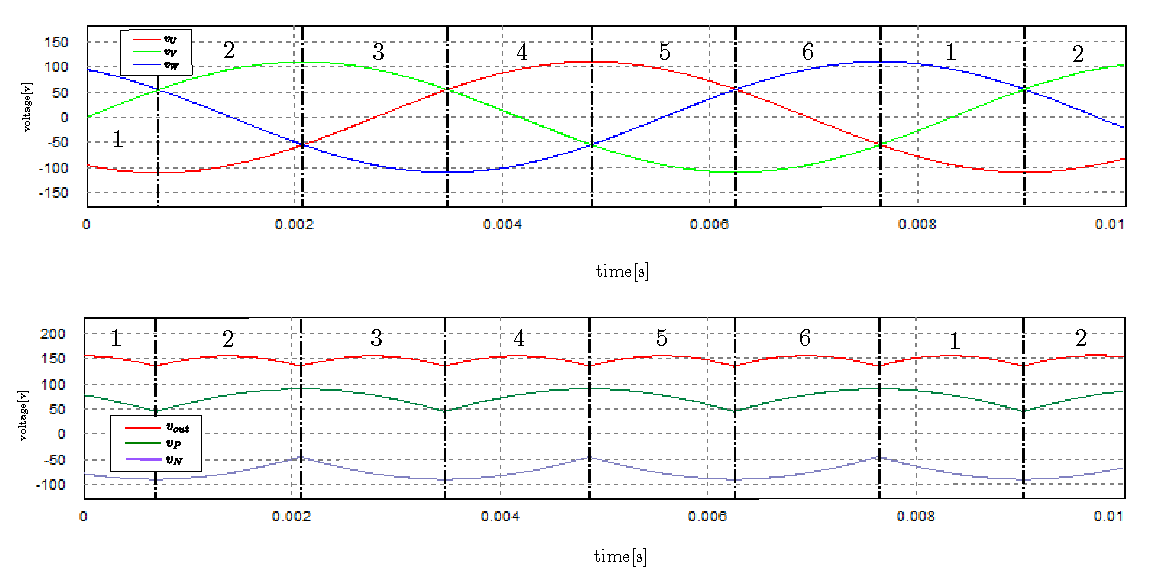
\includegraphics[scale=0.85]{../figure/waves.eps}\\
%  \hspace{0.0cm}
%  % 入力と出力\\
%  % \\
%  % \vspace{1.2cm}
%  % 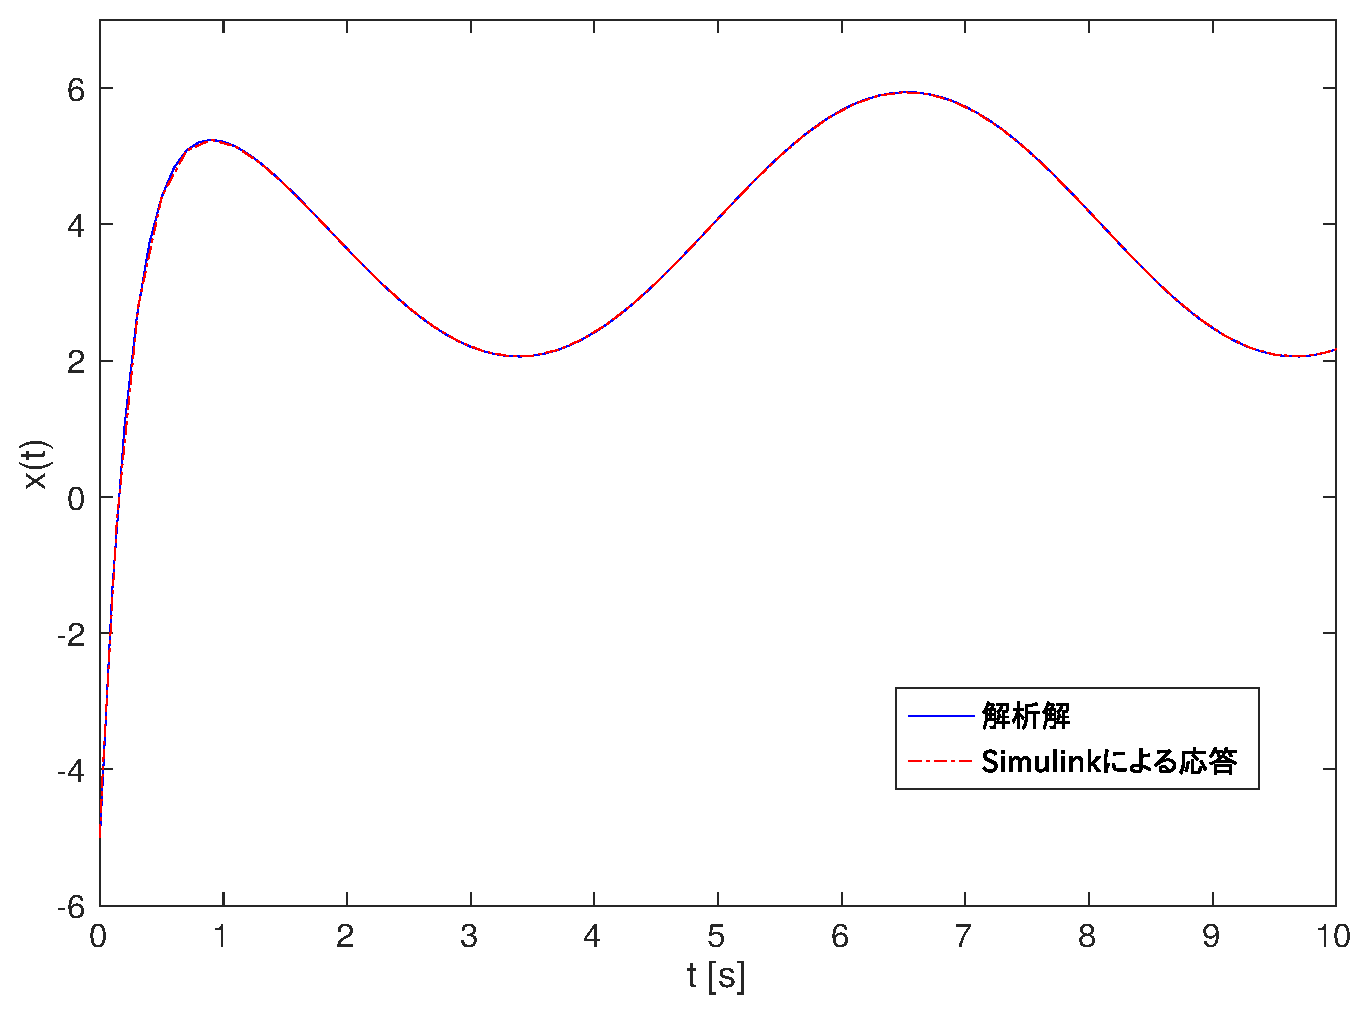
\includegraphics[scale=0.825]{../figure/output.eps}\\
%  % (b) 出力の電位\\
%  % \\
%  \caption{シミュレーションにより得られた各電源電圧(上)と出力電位(下)の波形}
%  \label{wave}
% \end{figure}

% \newpage

% % 図を並べて挿入

% \begin{figure}[tb]
%  \centering
%  \subfloat[区間1における回路動作]{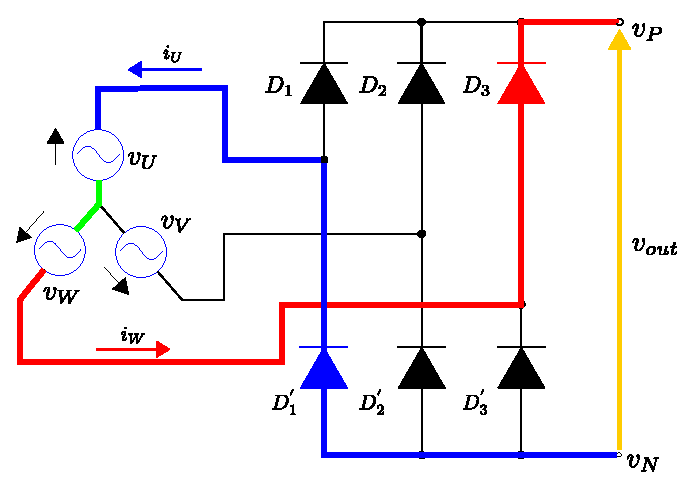
\includegraphics[scale=0.5]{../figure/kukan_1.eps}}
%  \hspace{1.5cm}
%  \subfloat[区間2における回路動作]{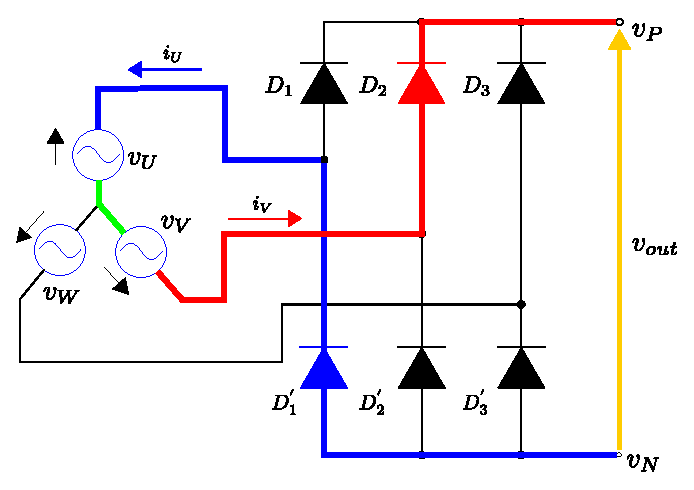
\includegraphics[scale=0.5]{../figure/kukan_2.eps}}
% \\
%  \vspace{0.5cm}
%  \subfloat[区間3における回路動作]{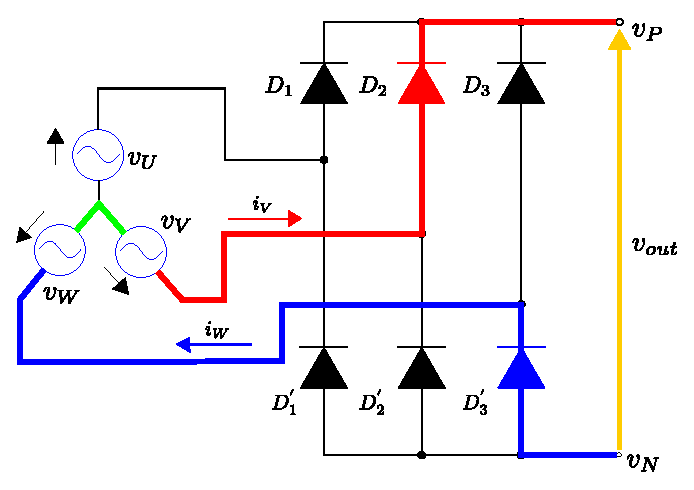
\includegraphics[scale=0.5]{../figure/kukan_3.eps}}
%  \hspace{1.5cm}
%  \subfloat[区間4における回路動作]{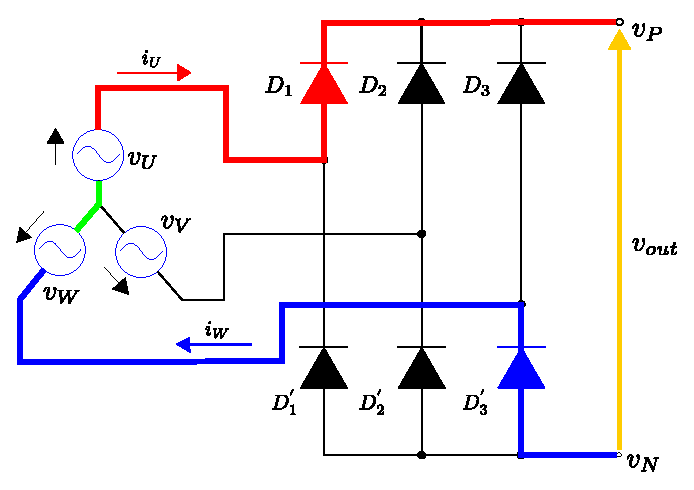
\includegraphics[scale=0.5]{../figure/kukan_4.eps}}
% \\
%  \vspace{0.5cm}
%  \subfloat[区間5における回路動作]{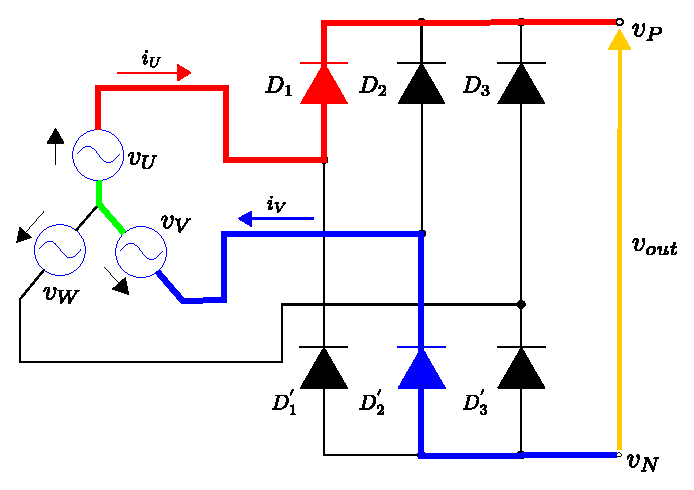
\includegraphics[scale=0.5]{../figure/kukan_5.eps}}
%  \hspace{1.5cm}
%  \subfloat[区間6における回路動作]{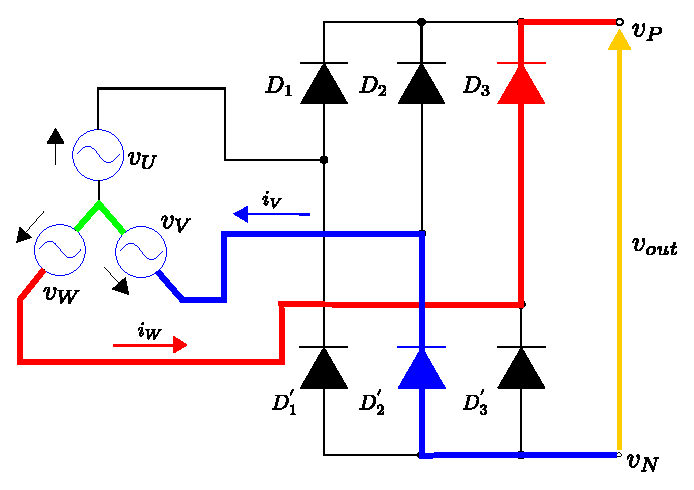
\includegraphics[scale=0.5]{../figure/kukan_6.eps}}
% \\
%  \caption{各区間での回路動作の様子}
%  \label{circuit_kaku}
% \end{figure}

% % 文中へのラベリング
% {\bf Fig. }\ref{circuit_kaku}に示す〜

% 参考文献
\begin{thebibliography}{99}
\addcontentsline{toc}{section}{参考文献}
\bibitem{1} 足立 修一・丸田 一郎,”カルマンフィルタの基礎”,東京電機大学出版局,pp.38-41,2012.
\bibitem{data} UCI Machine Learning Repositiry,SECOM Data Set,https://archive.ics.uci.edu/ml/datasets/SECOM,(最終閲覧日:2017年10月18日).
\end{thebibliography}

\end{document}
